\documentclass[conference]{IEEEtran}
\IEEEoverridecommandlockouts
\usepackage{cite}
\usepackage{amsmath,amssymb,amsfonts}
\usepackage{algorithmic}
\usepackage{graphicx}
\usepackage{textcomp}
\usepackage{xcolor}
\usepackage{algorithm}
\usepackage{algorithmic}
\usepackage{listings}
\def\BibTeX{{\rm B\kern-.05em{\sc i\kern-.025em b}\kern-.08em
    T\kern-.1667em\lower.7ex\hbox{E}\kern-.125emX}}
\begin{document}

\title{Formal Verification of Integer Multiplier Circuits\\}

\author{
\IEEEauthorblockN{Jonathan Wang}
\IEEEauthorblockA{\textit{Price College of Engineering} \\
\textit{University of Utah}\\
Salt Lake City, Utah \\
u1306458@utah.edu}
\and
\IEEEauthorblockN{Henry Silverman}
\IEEEauthorblockA{\textit{Price College of Engineering} \\
\textit{University of Utah}\\
Salt Lake City, Utah \\
henry.silverman@utah.edu}
\and
\IEEEauthorblockN{Garrett Slack}
\IEEEauthorblockA{\textit{Price College of Engineering} \\
\textit{University of Utah}\\
Salt Lake City, Utah \\
u1315263@utah.edu}
\and
\IEEEauthorblockN{Dmitry Panin}
\IEEEauthorblockA{\textit{Price College of Engineering} \\
\textit{University of Utah}\\
Salt Lake City, Utah \\
dmitry.panin@utah.edu}
}

\maketitle

\begin{abstract}
This paper employs advanced mathematical techniques, specifically polynomials, and ideals, 
to rigorously verify the correctness of an integer multiplier circuit. By leveraging algebraic methods, 
this approach will provide a deeper understanding of the circuit's behavior and enable a more robust 
verification process. 
\end{abstract}

\begin{IEEEkeywords}
polynomials, vanishing polynomials ($J_{0}$), ideals ($J$), multiplier circuit
\end{IEEEkeywords}

\section{Introduction}
In the field of digital circuit design, integer multiplier circuits stand as fundamental components with critical applications in various computing 
systems, ranging from embedded devices to high-performance computing architectures. The accurate and efficient operation of these multiplier 
circuits is crucial for ensuring the reliability and correctness of arithmetic computations. As technology advances and design complexities 
escalate, the need for rigorous verification methodologies has become increasingly pronounced to guarantee the integrity of digital circuits. Our 
project tests and verifies these integer multiplier circuits by employing the various methods studied in class on smaller circuits and circuits over fields.

\section{Approach}
Ideal membership testing is a great method to test and verify a 2-bit, 3-bit, 4-bit integer multiplier circuit.
We manually designed the 2-bit and 3-bit multiplier from scratch and generated the larger circuits utilizing the (.blif writing capabilities of the?) ABC synthesis tool. Next, we
converted the blif files to sing files using our parsing python script. The reverse topological term order (RTTO) was then derived from the circuit, and used to
represent the minimal Gröbner Basis. In digital circuit verification, there are several approaches to ensure a multiplier circuit implementation performs the same function as its specification. The first 
option could be creating a miter between the specification polynomials and the implementation, then checking if the Gröbner Basis (GB) is 1. Other approaches will be necessary at larger circuit sizes, 
such as weak Nullensatz, where the GB of the ideals and vanishing polynomials is 1 (GB($J$ + $J_{0}$) = 1). Another form of verification is checking if the Gröbner Basis of 
$J$ + $J_{0}$ equals 0 (GB($J$ + $J_{0}$) = 0).

\section{Process}
% the algorithms or techniques that you have studied, and you should demonstrate parts of your main contribution/study using example circuits, designs or code fragments
\subsection{Singular}
The Singular file consists of a ring, polynomials, ideals, and other code to define the behavior of a circuit and interpret its output. A ring is defined by properties, 
including the type of coefficients, number and names of variables, and arithmetic operations. The ordering of the inputs and outputs in 
the ring R should follow RTTO, consisting of the following order: outputs, internal gate outputs, and primary inputs. A polynomial (poly) is the algebraic representation of the logic in the circuit.
This can mean a poly is defined for each logic gate in the circuit or a more complex poly may be used to represent the functions of groups of gates. 
For example, $f_{spec}$ represents the desired mathematical functionality of the implemented circuit. Ideals are a subset of the polynomial ring 
that consists of all polynomials satisfying certain conditions. Vanishing polynomials are polynomials over a ring that output 0 for all elements in the ring.
Algorithm 1 shows the pseudo-code for an integer arithmetic circuit.
\begin{algorithm}
    \caption{Example Singular code for arithmetic circuit}
    \begin{algorithmic}
        \STATE // Declare ring
        \STATE ring R = 0, (outputs, internal outputs, inputs), lp;
        \STATE
        \STATE // Declare $f_{spec}$ and polys of internal gates
        \STATE poly $f_{spec}$ = specification equation of the circuit;
        \STATE //$f_{4}$ is an example of a polynomial describing gate behavior
        \STATE //z is an output, s and e are internal signals
        \STATE //z = $s_{0}$ - $e_{0}$ + 2*$s_{0}$*$e_{0}$
        \STATE poly $f_{4}$ = $z_{0}$ - $s_{0}$ - $e_{0}$ + 2*$s_{0}$*$e_{0}$; 
        \STATE //Continue to model logic gates over Q
        \STATE
        \STATE // Declare ideals
        \STATE ideal J = f4, f5,  f6, f7, f8, f9, f10, f11, f12, f13, f14, f15, f16;
        \STATE ideal J0 = vanishing polynomials;
        \STATE
        \STATE //Finding Gröbner Basis of the ideals plus the vanishing polynomials
        \STATE groebner($J$ + $J_{0}$);
        \STATE
        \STATE //Membership test using a condition checking statement to explicitly state membership
        \STATE NF($f_{spec}$, $J$ + $J_{0}$, 1);
    \end{algorithmic}
\end{algorithm}

\subsection{Singular results for 2-bit, 4-bit, and 16-bit multipliers}
First we tested the 2-bit multiplier for simplicity. If the Gröbner Basis of ideal {J} is 0 (empty), the variety of ideal {J} 
is empty or the miter is infeasible, shown in Fig. 1. 
\begin{figure}[ht]
    \centering
    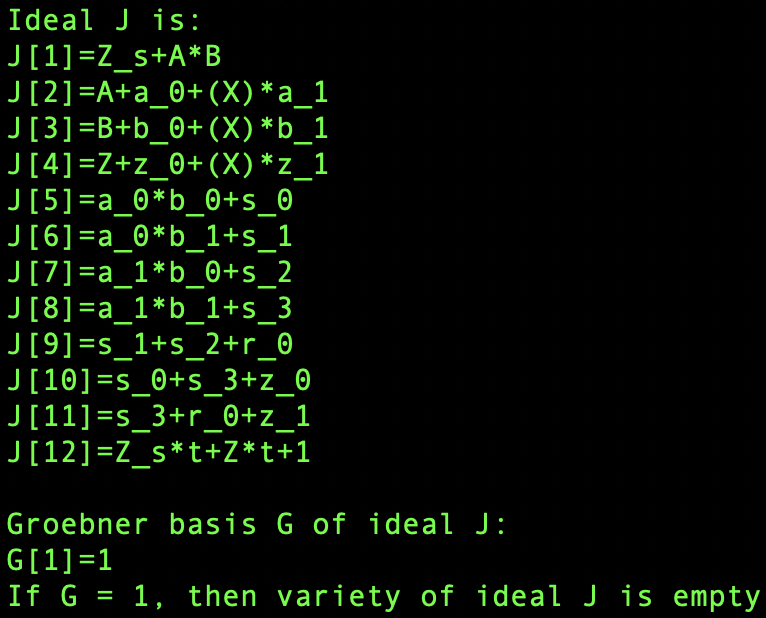
\includegraphics[scale = 0.5]{2-bit-GB1.png}
    \caption{Gröbner Basis = 1 without any bugs.}
\end{figure}
After introducing the bug(changing an AND gate to an OR gate), ideal {J} equals to 1, 
shown in Fig. 2. It means the variety is not empty, which also means solutions exist to ideal {J}.   
\begin{figure}[ht]
    \centering
    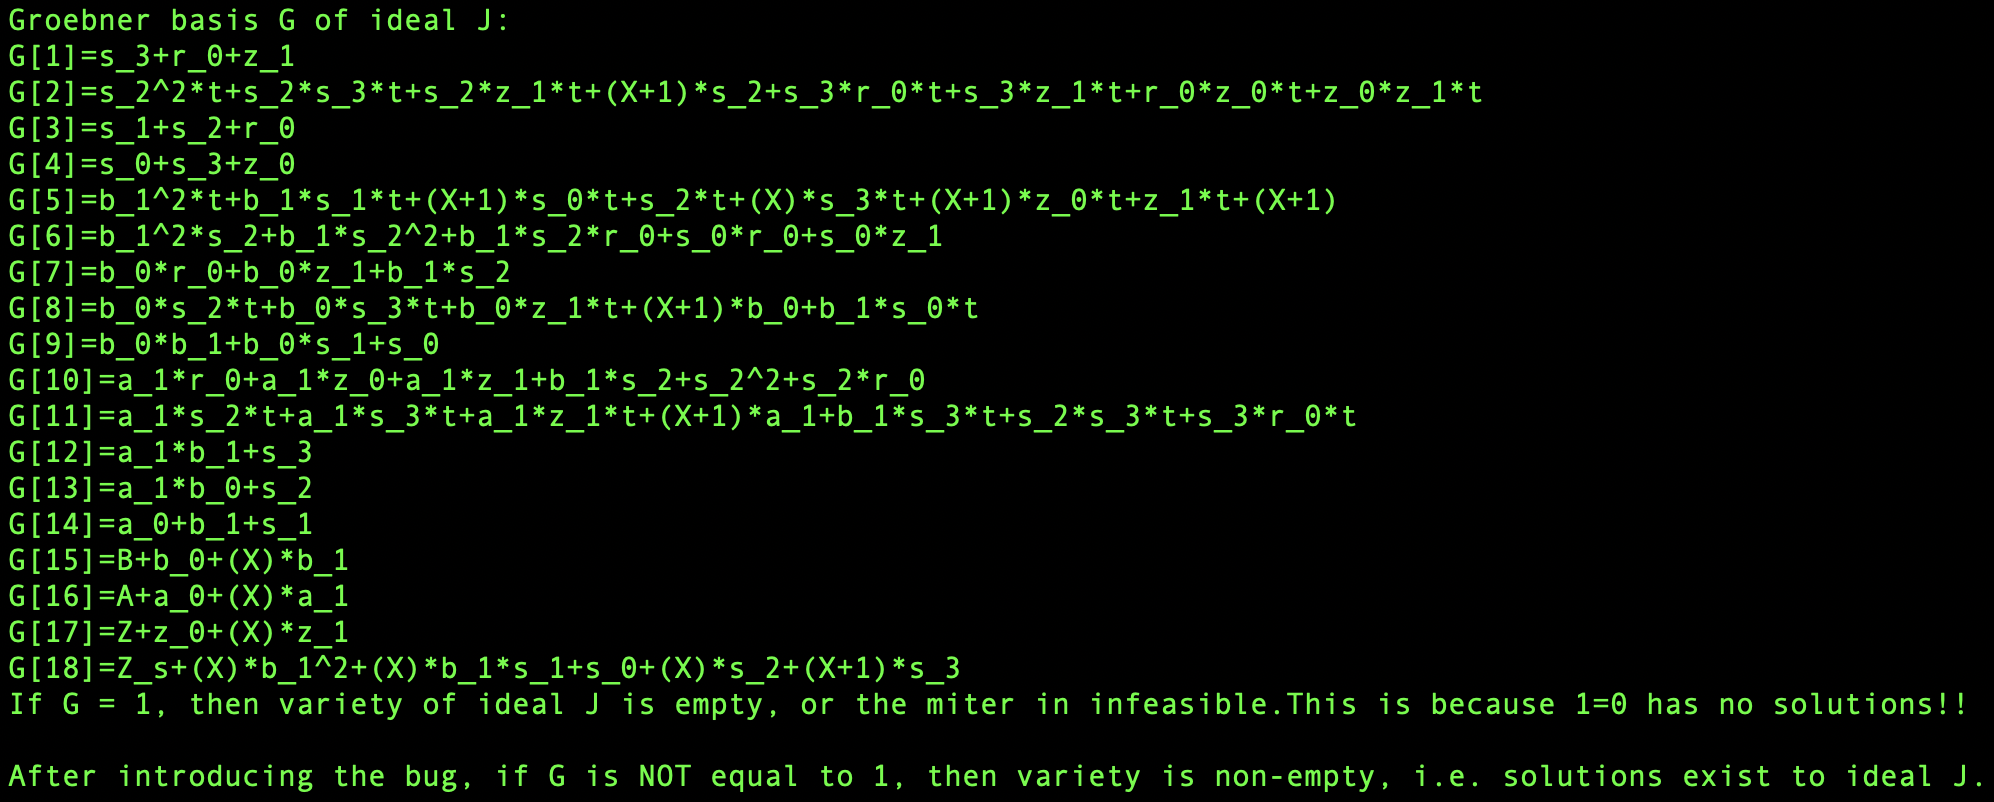
\includegraphics[scale = 0.25]{2-bit-GB2.png}
    \caption{Gröbner Basis = lots of polynomials = solutions exist.}
\end{figure}
Later, we introduced minimal and reduced Gröbner Basis for the larger 4-bit and 16-bit multiplier circuits. 
A minimal Gröbner basis is a special case of a Gröbner Basis that has the fewest number of elements possible 
while generating the same ideal. A reduced Gröbner Basis is a further refinement of the minimal Gröbner basis,
which means the leading coefficient of each polynomial is 1 and no monomial of another polynomial  is divisible 
by the leading monomial of another polynomial in the basis. 


\section{Algorithms and Techniques}
Techniques for ideal membership testing: 
\begin{enumerate}
    \item Setup the verification formulation over the polynomial ring R. 
    \item Declare a specification polynomial from circuit $f_{spec}$.
    \item Derive the polynomials from the gates of the circuit \{$f_{1}$, ..., $f_{s}$\}. 
    \item Set ideal J = $f_{1}$, ...,$f_{s}$.    
    \item Create the ideal of vanishing polynomials for each variable $J_{0}$
    \item Take the Gröbner Basis: G = GB(J + $J_{0}$).  
    \item The circuit implements \(f_{\text{spec}}\) \(\Longleftrightarrow\) \(f_{\text{spec}} \in (J + J_0)\) if and only if \(f_{\text{spec}}\)
    is divisible by G
\end{enumerate}
The steps to run Singular, ABC, and the Python script are provided in the README. 

\section{Software implementations} % needs to fix pseudocode cuz it doesnt work 
We implemented a Python function with assistance from ChatGPT to convert blif files to sing files. The code defines a gate mapping dictionary that maps gate types 
from the blif file to their corresponding names in Singular. It iterates through and searches for lines starting with '.gate' and extracts the gate type and its 
inputs, parsing and separating them accordingly into the Singular file. Additionally, we added code for error handling because the Singular file was empty when 
experimenting. Below is the pseudo-code for the Python file. 
\begin{lstlisting}
Function parse_blif_file(file_path):
Initialize gates, inputs, and outputs
  Open file_path
    For each line in file:
     If line starts with '.gate':
     Parse gate type, inputs, and output
     Replace 'new_n' with 'n' in input
     Add gate information to gates
     Update outputs and inputs set
     If line starts with '.inputs':
      Update inputs set
     If line starts with '.outputs':
      Update outputs set
  Return gates, inputs-outputs, outputs
    
Function topological_sort:
    Create a graph from gates
    Initialize order and visited sets
    Define topological sorting function
    For each output in graph:
     Visit(output)
    Return sorted order
    
Function generate_ring_declaration:
    Return ring declaration string
    
Function write_singular_file:
    Open output_path file
    Write ring declaration 
    Wtite polynomial equations
    Generate vanishing polynomials
    Write ideal declarations
    
Function main():
    Prompt user for BLIF file path
    Prompt user for output path
    Parse BLIF file
    Perform topological sort on gates
    Set ring size (default 2)
    Write .sing file
    Print completion message
    
Execute main()
\end{lstlisting}

\section{Concepts learned}
\subsection{Mathematical Ideals}
Ideals ensure the accuracy of electronic systems In circuit testing and verification. 
Ideal membership testing involves using mathematical 
models to assess whether a circuit aligns with specified ideal characteristics. 
Engineers compare these models with real-world circuit implementations to identify 
discrepancies to help detect potential faults in the design. This approach enhances 
precision and provides a systematic framework for validating complex circuits, 
contributing to the development of high-quality electronic systems.

\subsection{Gröbner Basis}
Gröbner Basis in-circuit testing and verification is a powerful method that 
involves algebraic techniques to analyze and validate complex electronic systems. 
Gröbner Bases provide a systematic way to address polynomial equations representing 
circuit behaviors. Gröbner Bases are a fundamental concept in algebraic geometry and 
computer algebra systems, and they play a crucial role in solving systems of polynomial 
equations. The primary idea behind Gröbner Bases is to provide a systematic method for 
transforming a set of polynomials into a more manageable and structured form.

\subsection{blif to sing conversion}
By using a python script to parse our mapped blif files (lib2.genlib), we 
can convert the list of gates contained in the blif file to a list of 
corresponding polynomials for our sing file. By splitting the blif file line by line and
parsing for key words such as ".gate," "XOR," "NAND," and "INV" to create the different
polynomial equations to model logic gates over Q. For example, "XOR" uses 
the equation z - a - b + 2ab, and "AND" uses the equation z = a * b for the 
corresponding polynomials. Python makes this very easy with its parsing functionalities. 

\subsection{Ideal Membership Testing}
Ideal membership testing is a mathematical approach used in circuit verification to 
determine whether a given circuit satisfies ideal properties or conditions. 
It involves algebraic structures known as ideals, particularly in the 
context of polynomial rings. An ideal is a subset of the polynomial ring that consists 
of all polynomials that satisfy certain conditions. In the context of circuit 
verification, the ideal encapsulates the set of polynomials representing the 
desired ideal behavior of the circuit. The core of the process involves determining 
whether a given polynomial, representing the behavior of the actual circuit, belongs 
to the ideal. If the polynomial is an element of the ideal, it indicates that the circuit 
satisfies the ideal properties. Otherwise, it suggests a deviation from the expected behavior.

\subsection{Miters}
Miters play a crucial role in circuit testing and verification. A model of the circuit is integrated into 
the testing process, allowing for comprehensive analysis. The miter compares the expected behavior with 
the actual circuit response using an xor gate to highlighting any discrepancies based on the model. 
By using miters, we can identify and address potential issues before moving to further stages of development 
or production, ensuring that the circuit functions as intended.  

\section{Labour Division}
\begin{itemize}
    \item Jonathan: Generated the blif files and converted it to Singular files and wrote the report
    \item Henry: Debugged Python Code and helped write report
    \item Garrett: Help write the report
    \item Dmitri: Provided Singular code for 2-bit,3-bit and 4-bit multipliers and visuals
\end{itemize}

\section{Conclusion}


\begin{thebibliography}{03}
\bibitem{b1} D. Ritirc, A. Biere and M. Kauers, "Column-wise verification of multipliers using computer algebra," 2017 Formal Methods in Computer Aided Design (FMCAD), Vienna, Austria, 2017, pp. 23-30, doi: 10.23919/FMCAD.2017.8102237.
\bibitem{b2} T. Pruss, P. Kalla and F. Enescu, "Efficient Symbolic Computation for Word-Level Abstraction From Combinational Circuits for Verification Over Finite Fields," in IEEE Transactions on Computer-Aided Design of Integrated Circuits and Systems, vol. 35, no. 7, pp. 1206-1218, July 2016, doi: 10.1109/TCAD.2015.2501301.
\bibitem{b3} Jerry R. Burch. 1991. Using BDDs to verify multipliers. In Proceedings of the 28th ACM/IEEE Design Automation Conference (DAC '91). Association for Computing Machinery, New York, NY, USA, 408–412. https://doi.org/10.1145/127601.127703
\end{thebibliography}
\vspace{12pt}

\end{document}
